\documentclass[12pt]{article}

\usepackage[utf8]{inputenc}
\usepackage{textcomp}

% -- support vietnamese --
\usepackage[vietnamese]{babel}
% -- support english --
% \usepackage[english]{babel}

\usepackage{float}
\usepackage{graphicx}
\usepackage{booktabs}
\usepackage[shortlabels]{enumitem}
\usepackage{emptypage}
\usepackage{subcaption}
\usepackage{multicol}
\usepackage[usenames, dvipsnames]{xcolor}

\usepackage{lipsum}
\usepackage{framed}
\usepackage{setspace}
\usepackage{extarrows}
\usepackage{scrextend}
\usepackage{commath}

% -- page set up --
\setlength{\parindent}{15pt}
\usepackage[a4paper,bindingoffset=0.2in,%
            left=1in,right=1in,top=1in,bottom=1in,%
            footskip=0.2in]{geometry}
\addtolength\footskip{1cm}

% -- math set up --
\usepackage{amsmath, amsfonts, mathtools, amsthm, amssymb}
\usepackage{mathrsfs}
\usepackage{cancel}
\usepackage{bbm}
\usepackage{bm}
\newcommand\N{\ensuremath{\mathbb{N}}}
\newcommand\R{\ensuremath{\mathbb{R}}}
\newcommand\Z{\ensuremath{\mathbb{Z}}}
\renewcommand\O{\ensuremath{\emptyset}}
\newcommand\Q{\ensuremath{\mathbb{Q}}}
\newcommand\C{\ensuremath{\mathbb{C}}}
\DeclareMathOperator{\sgn}{sgn}
\usepackage{systeme}
\let\svlim\lim\def\lim{\svlim\limits}
\let\implies\Rightarrow
\let\impliedby\Leftarrow
\let\iff\Leftrightarrow
\let\epsilon\varepsilon
\usepackage{stmaryrd} % for \lightning
\newcommand\contra{\scalebox{1.1}{$\lightning$}}

% -- correct --
\definecolor{correct}{HTML}{009900}
\newcommand\correct[2]{\ensuremath{\:}{\color{red}{#1}}\ensuremath{\to }{\color{correct}{#2}}\ensuremath{\:}}
\newcommand\green[1]{{\color{correct}{#1}}}

% -- horizontal rule --
\newcommand\hr{
    \noindent\rule[0.5ex]{\linewidth}{0.5pt}
}

% -- hide parts --
\newcommand\hide[1]{}

% -- tikz -- 
\usepackage{tikz}
\usepackage{tikz-cd}
\usetikzlibrary{intersections, angles, quotes, calc, positioning}
\usetikzlibrary{arrows.meta}
\usepackage{pgfplots}
\pgfplotsset{compat=1.13}
\tikzset{
    force/.style={thick, {Circle[length=2pt]}-stealth, shorten <=-1pt}
}

% -- Theorem set up --
\makeatother
\usepackage{thmtools}
\usepackage[framemethod=TikZ]{mdframed}
\mdfsetup{skipabove=1em,skipbelow=0em, innertopmargin=5pt, innerbottommargin=6pt}

\theoremstyle{definition}

\makeatletter

\@ifclasswith{report}{nocolor}{
    \declaretheoremstyle[headfont=\bfseries\sffamily, bodyfont=\normalfont, mdframed={ nobreak } ]{thmgreenbox}
    \declaretheoremstyle[headfont=\bfseries\sffamily, bodyfont=\normalfont, mdframed={ nobreak } ]{thmredbox}
    \declaretheoremstyle[headfont=\bfseries\sffamily, bodyfont=\normalfont]{thmbluebox}
    \declaretheoremstyle[headfont=\bfseries\sffamily, bodyfont=\normalfont]{thmblueline}
    \declaretheoremstyle[headfont=\bfseries\sffamily, bodyfont=\normalfont, numbered=no, mdframed={ rightline=false, topline=false, bottomline=false, }, qed=\qedsymbol ]{thmproofbox}
    \declaretheoremstyle[headfont=\bfseries\sffamily, bodyfont=\normalfont, numbered=no, mdframed={ nobreak, rightline=false, topline=false, bottomline=false } ]{thmexplanationbox}
    \AtEndEnvironment{eg}{\null\hfill$\diamond$}%
}{
    \declaretheoremstyle[
        headfont=\bfseries\sffamily\color{ForestGreen!70!black}, bodyfont=\normalfont,
        mdframed={
            linewidth=2pt,
            rightline=false, topline=false, bottomline=false,
            linecolor=ForestGreen, backgroundcolor=ForestGreen!10,
        }
    ]{thmgreenbox}

    \declaretheoremstyle[
        headfont=\bfseries\sffamily\color{NavyBlue!70!black}, bodyfont=\normalfont,
        mdframed={
            linewidth=2pt,
            rightline=false, topline=false, bottomline=false,
            linecolor=NavyBlue, backgroundcolor=NavyBlue!5,
        }
    ]{thmbluebox}

    \declaretheoremstyle[
        headfont=\bfseries\sffamily\color{NavyBlue!70!black}, bodyfont=\normalfont,
        mdframed={
            linewidth=2pt,
            rightline=false, topline=false, bottomline=false,
            linecolor=NavyBlue
        }
    ]{thmblueline}

    \declaretheoremstyle[
        headfont=\bfseries\sffamily\color{RawSienna!70!black}, bodyfont=\normalfont,
        mdframed={
            linewidth=2pt,
            rightline=false, topline=false, bottomline=false,
            linecolor=RawSienna, backgroundcolor=RawSienna!10,
        }
    ]{thmredbox}

    \declaretheoremstyle[
        headfont=\bfseries\sffamily\color{RawSienna!70!black}, bodyfont=\normalfont,
        numbered=no,
        mdframed={
            linewidth=2pt,
            rightline=false, topline=false, bottomline=false,
            linecolor=RawSienna, backgroundcolor=RawSienna!1,
        },
        qed=\qedsymbol
    ]{thmproofbox}

    \declaretheoremstyle[
        headfont=\bfseries\sffamily\color{NavyBlue!70!black}, bodyfont=\normalfont,
        numbered=no,
        mdframed={
            linewidth=2pt,
            rightline=false, topline=false, bottomline=false,
            linecolor=NavyBlue, backgroundcolor=NavyBlue!1,
        },
    ]{thmexplanationbox}
}

% -- use for english --

\declaretheorem[style=thmgreenbox, name=Definition]{definition}
\declaretheorem[style=thmbluebox, numbered=no, name=Example]{eg}
\declaretheorem[style=thmbluebox, numbered=no, name=Exercise]{ex}
\declaretheorem[style=thmredbox, name=Proposition]{prop}
\declaretheorem[style=thmredbox, name=Theorem]{theorem}
\declaretheorem[style=thmredbox, name=Lemma]{lemma}
\declaretheorem[style=thmredbox, numbered=no, name=Corollary]{corollary}

\@ifclasswith{report}{nocolor}{
    \declaretheorem[style=thmproofbox, name=Proof]{replacementproof}
    \declaretheorem[style=thmexplanationbox, name=Proof]{explanation}
    \renewenvironment{proof}[1][\proofname]{\begin{replacementproof}}{\end{replacementproof}}
}{
    \declaretheorem[style=thmproofbox, name=Proof]{replacementproof}
    \renewenvironment{proof}[1][\proofname]{\vspace{-10pt}\begin{replacementproof}}{\end{replacementproof}}

    \declaretheorem[style=thmexplanationbox, name=Proof]{tmpexplanation}
    \newenvironment{explanation}[1][]{\vspace{-10pt}\begin{tmpexplanation}}{\end{tmpexplanation}}
}

% -- use for vietnamese --

\declaretheorem[style=thmgreenbox, name=Định nghĩa]{defivn}
\declaretheorem[style=thmbluebox, numbered=no, name=Ví dụ]{egvn}
\declaretheorem[style=thmbluebox, numbered=no, name=Bài tập]{exvn}
\declaretheorem[style=thmredbox, name=Mệnh đề]{propvn}
\declaretheorem[style=thmredbox, name=Định lý]{theovn}
\declaretheorem[style=thmredbox, name=Bổ đề]{lemmavn}
\declaretheorem[style=thmredbox, numbered=no, name=Hệ quả]{corollaryvn}
\declaretheorem[style=thmblueline, numbered=no, name=Nhận xét]{remarkvn}

\declaretheorem[style=thmexplanationbox, name=Giải]{replacementsolvevn}
\newenvironment{solvevn}[1][\proofname]{\vspace{-10pt}\begin{replacementsolvevn}}{\end{replacementsolvevn}}

\@ifclasswith{report}{nocolor}{
    \declaretheorem[style=thmproofbox, name=Chứng minh]{replacementproofvn}
    \newenvironment{proofvn}[1][\proofname]{\begin{replacementproofvn}}{\end{replacementproofvn}}
}{
    \declaretheorem[style=thmproofbox, name=Chứng minh]{replacementproofvn}
    \newenvironment{proofvn}[1][\proofname]{\vspace{-10pt}\begin{replacementproofvn}}{\end{replacementproofvn}}
}

\newtheorem*{probvn}{Bài toán}


% ------------------------

\makeatother

\declaretheorem[style=thmblueline, numbered=no, name=Remark]{remark}
\declaretheorem[style=thmblueline, numbered=no, name=Note]{note}

\newtheorem*{uovt}{UOVT}
\newtheorem*{notation}{Notation}
\newtheorem*{previouslyseen}{As previously seen}
\newtheorem*{problem}{Problem}
\newtheorem*{observe}{Observe}
\newtheorem*{property}{Property}
\newtheorem*{intuition}{Intuition}

%%%%% something else %%%%%%%%%%%%%%%%%%
\usepackage{etoolbox}
% \AtEndEnvironment{vb}{\null\hfill$\diamond$}%
% \AtEndEnvironment{intermezzo}{\null\hfill$\diamond$}%
% \AtEndEnvironment{opmerking}{\null\hfill$\diamond$}%

% http://tex.stackexchange.com/questions/22119/how-can-i-change-the-spacing-before-theorems-with-amsthm
\makeatletter
\def\thm@space@setup{%
  \thm@preskip=\parskip \thm@postskip=0pt
}

%%%%%% Header/Footer %%%%%%%%%%%%%%%%%%
\usepackage{fancyhdr}
\pagestyle{fancy}
\fancyhf{}
\rfoot[]{Trang \thepage}
% \lfoot[]{\rightmark}
\lhead[]{}
% \rhead[]{\leftmark}
\makeatother
%%%%%%%%%%%%%%%%%%%%%%%%%%%%%%%%%%%%%%%

%%%%%%%%%%%%% inkscape %%%%%%%%%%%%%%%%
\usepackage{import}
\usepackage{xifthen}
\pdfminorversion=7
\usepackage{pdfpages}
\usepackage{transparent}
\newcommand{\incfig}[1]{%
    \def\svgwidth{\columnwidth}
    \import{./figures/}{#1.pdf_tex}
}
%%%%%%%%%%%%%%%%%%%%%%%%%%%%%%%%%%%%%%%

% %http://tex.stackexchange.com/questions/76273/multiple-pdfs-with-page-group-included-in-a-single-page-warning
\pdfsuppresswarningpagegroup=1

%%%%%%% url setup %%%%%%%%%%%%%%%%%%%%%
\usepackage{hyperref}
\hypersetup{
    colorlinks=true,
    urlcolor=cyan,
    linkcolor=red,
}
%%%%%%%%%%%%%%%%%%%%%%%%%%%%%%%%%%%%%%%

%%%%% chapter and section %%%%%%%%%%%%%
\newcommand{\nchapter}[2]{%
    \setcounter{chapter}{#1}%
    \addtocounter{chapter}{-1}%
    \chapter{#2}
}

\newcommand{\nsection}[3]{%
    \setcounter{chapter}{#1}%
    \setcounter{section}{#2}%
    \addtocounter{section}{-1}%
    \section{#3}
}
%%%%%%%%%%%%%%%%%%%%%%%%%%%%%%%%%%%%%%%

%%%%% something else %%%%%%%%%%%%%%%%%%
\usepackage{faktor}

\makeatletter
\DeclareRobustCommand*{\mfaktor}[3][]
{
   { \mathpalette{\mfaktor@impl@}{{#1}{#2}{#3}} }
}
\newcommand*{\mfaktor@impl@}[2]{\mfaktor@impl#1#2}
\newcommand*{\mfaktor@impl}[4]{
   \settoheight{\faktor@zaehlerhoehe}{\ensuremath{#1#2{#3}}}%
   \settoheight{\faktor@nennerhoehe}{\ensuremath{#1#2{#4}}}%
      \raisebox{-0.5\faktor@zaehlerhoehe}{\ensuremath{#1#2{#3}}}%
      \mkern-4mu\diagdown\mkern-5mu%
      \raisebox{0.5\faktor@nennerhoehe}{\ensuremath{#1#2{#4}}}%
}
\makeatother
%%%%%%%%%%%%%%%%%%%%%%%%%%%%%%%%%%%%%%%

%%%% icon support %%%%
\usepackage{fontawesome5} 

\usepackage{listings}
\usepackage{algorithm}
\usepackage{algpseudocode}

\definecolor{codegreen}{rgb}{0,0.6,0}
\definecolor{codegray}{rgb}{0.5,0.5,0.5}
\definecolor{codepurple}{rgb}{0.58,0,0.82}
\definecolor{backcolour}{rgb}{0.95,0.95,0.92}

\lstdefinestyle{mystyle}{
    backgroundcolor=\color{backcolour},   
    commentstyle=\color{codegreen},
    keywordstyle=\color{magenta},
    numberstyle=\tiny\color{codegray},
    stringstyle=\color{codepurple},
    basicstyle=\ttfamily\footnotesize,
    breakatwhitespace=false,         
    breaklines=true,                 
    captionpos=b,                    
    keepspaces=true,                 
    numbers=left,                    
    numbersep=5pt,                  
    showspaces=false,                
    showstringspaces=false,
    showtabs=false,                  
    tabsize=2
}

\lstset{style=mystyle}

\title{Bài tập thực hành Tuần 1\\
Môn: Phương pháp Toán cho Trí tuệ nhân tạo}
\author{Lê Nguyễn - 21120511}

\begin{document}
\maketitle

%%%%%%%%%%
\textbf{Bài 1:}
\begin{itemize}
    \item[(a)] Ta có:
    $$
    \begin{aligned}
        g(n) = (3n + \dfrac{1}{\sqrt{n}})(4n - \sqrt{n}) &= 12n^2 - 3n\sqrt{n} + 4\sqrt{n} - 1 \\
        &= 12n^2 + \sqrt{n}(4 - 3n) - 1
    \end{aligned}
    $$

    \item[] Ta thấy:
    $$
    n^2 \leq 12n^2 + \sqrt{n}(4 - 3n) - 1 \leq 50n^2, \hspace*{10pt} \forall x \geq 0.063
    $$

    \item[] Do đó $g(n) \in \Theta(n^2)$.
    
    \begin{figure}[H]
        \centering
        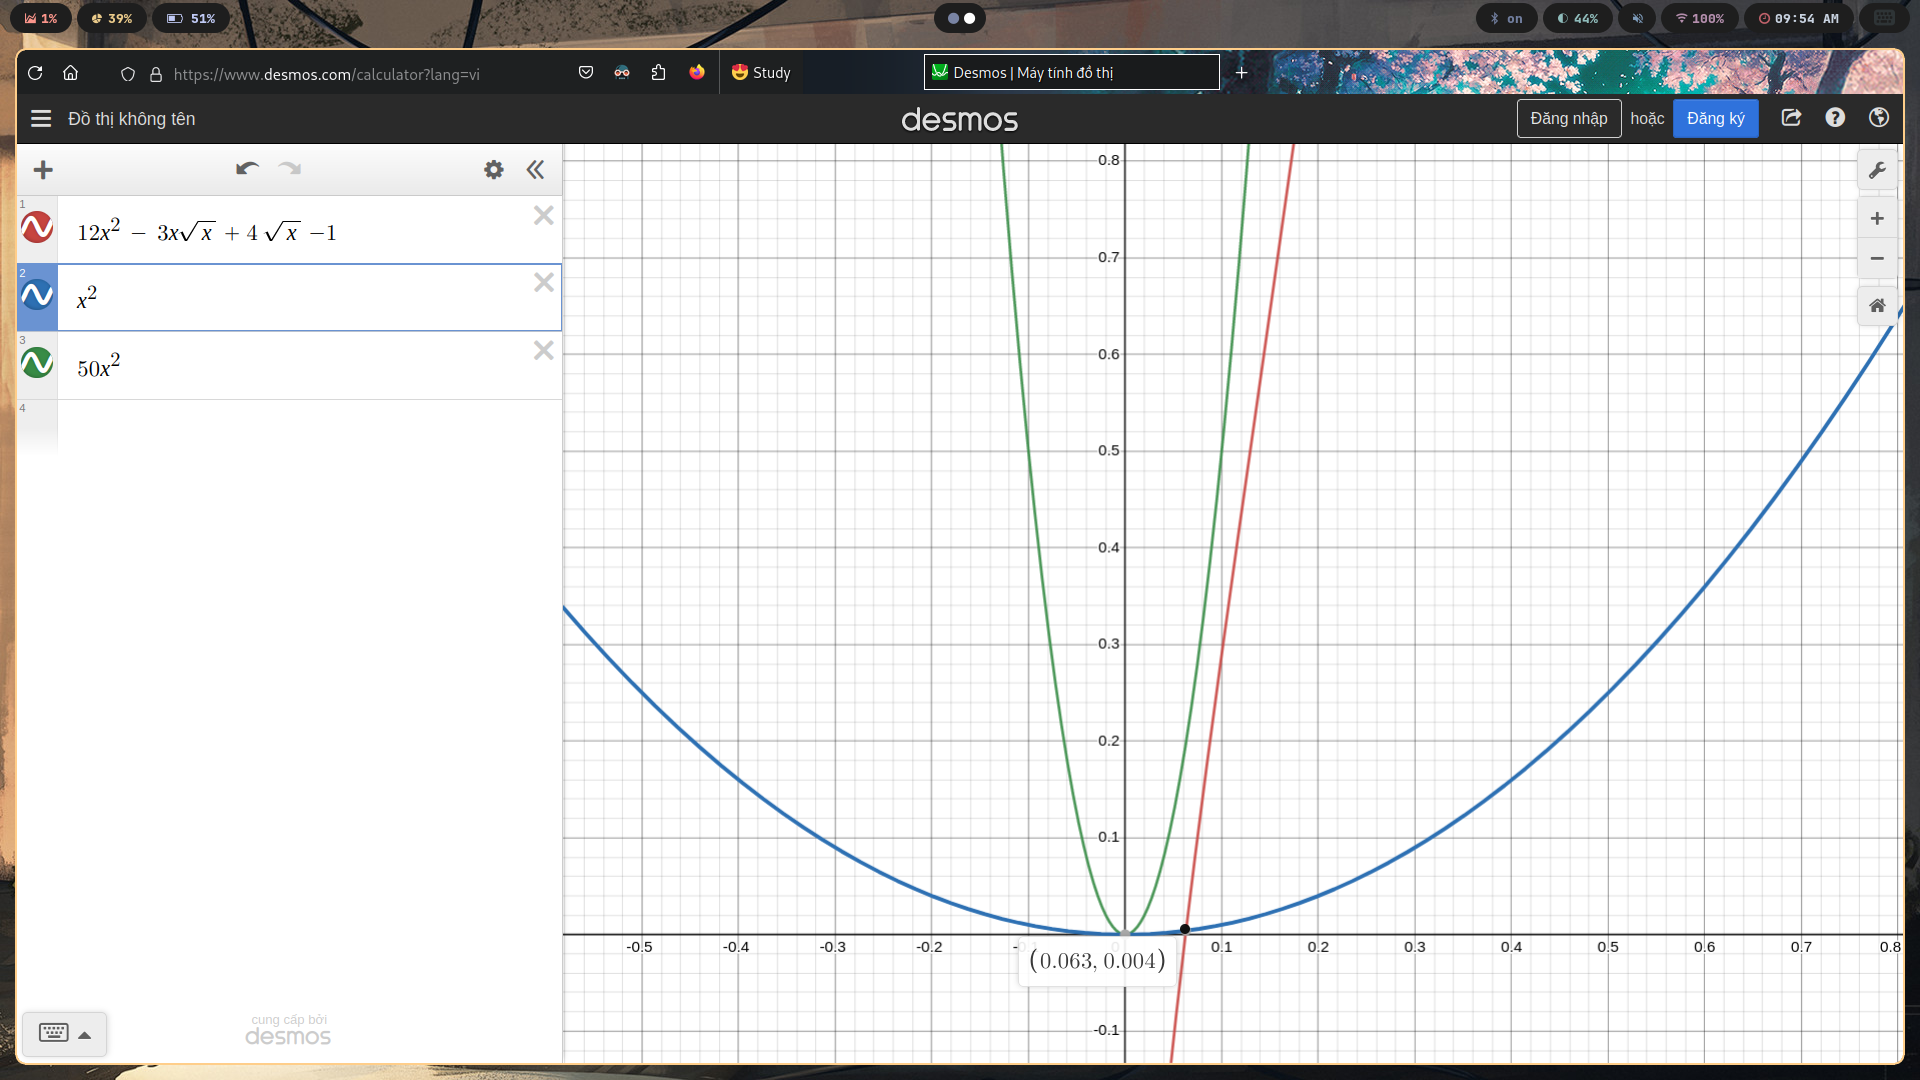
\includegraphics[scale=0.23]{1677725662.png}
    \end{figure}

    % \item[(b)] Xét một phần tử $a$ bất kì nằm trong $\Omega(n^3)$. Do $a \geq n^3$ nên $a \geq n^2$. Vì vậy $a \in \Omega(n^2)$. Vậy $\Omega(n^3) \subseteq \Omega(n^2)$.

    \item[(b)] Xét hàm số $f(n)$ bất kì thuộc $\Omega(n^3)$, ta có:
    $$
    f(n) \geq c_0n^3, \hspace*{10pt} \forall n \geq n_0
    $$

    \item[] Khi đó tồn tại cặp số $(c_1, n_0)$ sao cho:
    $$
    f(n) \geq c_0n^3 \geq c_1n^2 \hspace*{10pt} \forall n \geq n_0
    $$

    \item[] Do đó $f(n) \in \Omega(n^2)$. Vậy $\Omega(n^3) \subseteq \Omega(n^2)$.
\end{itemize}
\vspace*{10pt}

%%%%%%%%%%
\textbf{Bài 2:}
\begin{itemize}
    \item[(a)] Đặt thời gian chạy của cả chương trình là $T(n)$ và $t_i$ là số lần chạy của vòng for lồng phía trong. Ứng với mỗi dòng ta sẽ mất đi $c_i$ tài nguyên với $i$ là số dòng.

    \item[] Ta có: 
    \begin{itemize}
        \item Dòng đầu tiên (bắt đầu từ vòng for đầu tiên) mất $c_1 \left(\dfrac{n}{3} + 2\right)$
        \item Dòng thứ hai mất:
        $$
        c_2\sum_{i=1}^{n/3 + 1}t_i = c_2 \left(\dfrac{n}{3}+1\right)t_i \hspace*{10pt} \text{(do vòng for thứ hai không phụ thuộc vào $i$)}
        $$
        \item Dòng thứ ba mất:
        $$
        c_3\sum_{i=1}^{n/3+1}(t_i - 1) = c_3 \left(\dfrac{n}{3} + 1\right)(t_i - 1)
        $$
    \end{itemize}

    \item[] Kết hợp cả 3 và ta biết $t_i = \left \lfloor \dfrac{n}{4} + 1 \right \rfloor + 1$, ta được:
    $$
    \begin{aligned}
    T(n) &= c_1\left(\dfrac{n}{3} + 2\right) + c_2\left(\dfrac{n}{3} + 1 \right)\left(\dfrac{n}{4} + 2\right) + c_3\left(\dfrac{n}{3} + 1\right)\left(\dfrac{n}{4} + 1\right) \\
    &= \left(\dfrac{c_2}{12} + \dfrac{c_3}{12}\right)n^2 + \left(\dfrac{c_1}{3} + \dfrac{3c_2}{4} + \dfrac{5c_3}{12}\right)n  + 2c_1 + 2c_2 + c_3
    \end{aligned}
    $$

    \item[$\Rightarrow$] Do là một hàm bậc 2 nên thời gian chạy là $\Theta(n^2)$.

    \item[(b)] Đặt tương tự như câu $a$, ta có:
    \begin{itemize}
        \item Dòng đầu tiên ta mất $c_1(n+1)$.
        \item Dòng thứ hai mất:
        $$
        c_2\sum_{i=1}^{n}t_i
        $$

        \item Dòng thứ ba mất:
        $$
        c_3\sum_{i=1}^n(t_i - 1)
        $$
    \end{itemize}
    
    \item[] Dựa theo câu $a$ ta có được $t_i = \left \lfloor \dfrac{n}{i} + 1 \right \rfloor + 1$

    \item[] Xét 2 tổng ta được:
    $$
    \begin{aligned}
    \sum_{i=1}^n t_j &= \sum_{i=1}^n \left( \dfrac{n}{i} + 2 \right) \\
    &= n + \dfrac{n}{2} + ... + 1 + 2n \\
    &= n \left(\sum_{i=1}^n \dfrac{1}{i} \right) + 2n
    \end{aligned}
    $$
    và  
    $$
    \begin{aligned}
    \sum_{i=1}^n (t_j - 1) &= \sum_{i=1}^n \left( \dfrac{n}{i} + 1 \right) \\
    &= n + \dfrac{n}{2} + ... + 1 + n \\
    &= n \left( \sum_{i=1}^n \dfrac{1}{i} \right) + n
    \end{aligned}
    $$

    \item[] Chuỗi $\displaystyle \sum_{i=1}^n \frac{1}{i}$ còn được gọi là số Harmonic và có giá trị xấp xỉ là $\ln(n)$.

    \item[] Vậy kết hợp lại ta được:
    $$
    c_1(n+1) + c_2(n\ln(n) + 2n) + c_3(n\ln(n) + n)
    $$

    \item[$\implies$] Vậy độ phức tạp của thuật toán trên là $\Omega(n\ln(n))$ 
    
    \begin{note}
    Do số Harmonic là xấp xỉ xuống và bỏ các thành phần liên quan nên khi chạy thực tế thì số lần chạy sẽ cao hơn $n\ln(n)$ nên em chọn $\Omega$, đồng thời qua nhiều lần dùng máy tính chạy thử (chạy tới $n = 10000000$) thì em thấy vẫn đúng.
    \end{note}
\end{itemize}
\vspace*{10pt}

%%%%%%%%%%
\textbf{Bài 3:} 
\begin{itemize}
    \item[(a)] $O(n^2)$.

    \item Mục đích của ta là lấy tổng số phần tử của mảng trừ đi số phần tử bị lặp thì sẽ được số phần tử phân biệt có trong mảng.

    \item Để tìm được số phần tử bị lặp. Ta tạo một biến \textbf{count} để lưu số phần tử bị lặp.

    \item Sau đó ta chạy vòng lặp cho $i$ từ $1$ đến $n-1$ và một vòng lặp phía trong cho $j$ chạy từ $0$ đến $i-1$. Nếu có phần tử $A[j]$ nào bằng với $A[i]$ thì ta tăng biến \textbf{count} lên 1.
    
    \item Sau khi kết thúc vòng lặp ta chỉ cần lấy độ dài của mảng trừ cho \textbf{count}.

\begin{lstlisting}[language=Python]
from typing import List

def CountDistinct(A: List[int]) -> int:
    count: int = 0
    n: int = len(A)

    for i in range(1, n):
        for j in range(0, i):
            if (A[j] == A[i]) 
                count = count + 1

    return n - count
\end{lstlisting}

\item Trong lúc chạy ta không tạo ra mảng phụ nên độ phức tạp không gian là $O(1)$.

\item[(b)] $O(n\log n)$.

\item Ở cách này, đầu tiên ta sẽ sắp xếp lại các phần tử trong mảng dùng phép sắp xếp có độ phức tạp là $O(n \log n)$ và để tối ưu nhất ta dùng \textbf{Quick Sort} (bởi vì \textbf{Merge Sort} sẽ tạo ra array phụ trong lúc sắp xếp).

\item Sau đó ta lặp mảng $A$ từ đầu đến cuối. Nếu phần tử trước khác phần tử sau thì ta sẽ tăng biến count lên 1.

\item Khi đó biến count chính là só phần tử phân biệt trong mảng.

\begin{lstlisting}[language=Python]
from typing import List

def Partition(A: List[int], low: int, high: int) -> int:
    pivot: int = A[high]
    i: int = low - 1

    for j in range(low, high):
        if (A[j] <= pivot):
            i = i + 1
            (A[i], A[j]) = (A[j], A[i])

    (A[i+1], A[high]) = (A[high], A[i+1])

    return i + 1

def QuickSort(A: List[int], low: int, high: int) -> None:
    if (low < high):
        p = Partition(A, low, high)
        QuickSort(A, low, p - 1)
        QuickSort(A, p + 1, high)

def CountDistinct(A: List[int]) -> int:
    count: int = 0
    n: int = len(A)

    QuickSort(A, 0, n-1)

    for i in range(n-1):
        if (A[i] != A[i+1]):
            count = count + 1

    return count
\end{lstlisting}

\item Trong lúc chạy ta không tạo ra mảng phụ nên độ phức tạp không gian là $O(1)$.

\item[(c)] $O(n)$.

\item Ở cách này, đầu tiên ta sẽ tạo một array mới (gọi là mảng $B$) có độ dài bằng với độ lớn của phần tử lớn nhất trong mảng cần xét (gọi là mảng $A$) cộng thêm 1.

\item Sau đó ta lặp qua mảng $A$ thí dụ $A$ có phần tử $7$ thì $B[7]$ tăng thêm 1. Ta sẽ làm quy luật như vậy cho đến hết mảng. 

\item Cuối cùng ta chỉ cần lặp qua mảng $B$, nếu có phần tử nào lớn hơn $0$ thì ta tăng thêm $1$ vào biến count. Và cuối cùng thì biến count chính là số phần tử phân biệt trong mảng.

\item Ngoài ra để chắc chắn thuật toán chạy đúng, ta lấy mỗi phần tử trong $A$ trừ cho phần tử nhỏ nhất trong $A$, khi đó trong $A$ sẽ không có phần tử nào bị âm.

\begin{lstlisting}[language=Python]
from typing import List

def CountDistinct(A: List[int]) -> int:
    count: int = 0
    n: int = len(A)

    minA: int = min(A)

    # tru cac phan tu trong A cho min(A) de khong co phan tu nao < 0
    for k in range(0, n):
        A[k] = A[k] - minA

    # tao mang B gom cac phan tu la 0 va co do dai = max(A)
    B: List[int] = [0] * (max(A) + 1)
    m: int = len(B)

    for i in range(0, n):
        B[A[i]] = B[A[i]] + 1

    for j in range(0, m):
        if (B[j] > 0):
            count = count + 1

    return count
\end{lstlisting}

\item Do trong quá trình chạy tạo thêm mảng phụ $B$ nên có độ phức tạp không gian là $O(n)$. 

\item Nếu dựa theo thuật toán trên mảng $B$ có tối đa là $10^4$ phần tử và mỗi phần tử sẽ nằm trong khoảng $[0, 2.10^4]$. Và thuật toán này chỉ áp dụng cho số nguyên.

\end{itemize}

\vspace*{10pt}

%%%%%%%%%%
\textbf{Bài 4 (1):}
\begin{itemize}
    \item Đầu tiên ta xem xét giá trị của $n$, nếu $n < 8$ thì ta sẽ trả về gía trị $n$, do khi $n < 8$ thì cách phân hoạch duy nhất là phân hoạch thành $n$ số 1.

    \item Nếu $n > 8$ thì ta tìm số lớn nhất mà $n$ có thể phân hoạch được. Ví dụ nếu $n = 84$ thì số lớn nhất mà $n$ có thể phân hoạch được là $4$, do $4^3 = 64 < 84$ nhưng $5^3 = 125 > 84$. 
    
    \item Cách tìm số lớn nhất này ta chỉ cần lặp $i$ từ $1 \to 100$ (do giới hạn là $10^6$ mà $100^3$ cũng bằng $10^6$). Tạo một biến \textbf{largest} tăng thêm 1 sau mỗi lần lặp, nếu lặp đến một số mũ 3 lớn hơn $n$ thì ta thoát lặp, nếu lặp đến số mũ 3 bằng $n$ thì ta được kết quả là $1$ (do đó là cách phân hoạch $n$ ít nhất).

    \item Sau đó ta tạo một mảng phụ để lưu số phần tử của các cách phân hoạch $n$ có thể.

    \item Sau đó ta giảm dần largest để tìm số phần tử của các lần phân hoạch $n$, hàm này nhận tham số là $n$ và \textbf{largest}. Cách hoạt động như sau:

    \begin{itemize}
        \item Xét ví dụ là $n = 84$ ta có được \textbf{largest} $= 4$.

        \item Ta tạo biến \textbf{numOfPartition} để lưu giữ số phần tử của lần phân hoạch, ban đầu là $0$.

        \item Đầu tiên ta thấy $n > \textbf{largest}^3$ nên ta được phần tử đầu tiên của phần hoạch là $4^3$ và $n$ còn lại $84 - 4^3 = 84 - 64 = 20$. Cuối cùng ta cộng \textbf{numOfPartition} lên 1.

        \item Lần lặp tiếp theo ta thấy $n < \textbf{largest}^3$ nên ta giảm \textbf{largest} xuống 1 còn 3. Tiếp theo ta cũng thấy $n < \textbf{largest}^3$ nên giảm \textbf{largest} xuống 1 còn 2.

        \item Lần lặp này ta thấy $n > \textbf{largest}^3$ nên phần tử tiếp theo của phân hoạch là $2^3$ và $n$ còn lại $20 - 2^3 = 20 - 8 = 12$. Lúc này \textbf{numOfPartition} được 2. Tương tự lần lặp tiếp theo ta có $n$ còn lại là $12 - 2^3 = 12 - 8 = 4$. Lúc này \textbf{numOfPartition} lên 3.

        \item Lần lặp cuối ta thấy $n < \textbf{largest}^3$ nên giảm \textbf{largest} xuống còn 1 và vòng while thực hiện xong.

        \item Sau khi thoát khỏi vòng while ta thấy $n$ vẫn còn sót lại và $n < 8$ ($n = 4$) nên số phần tử trong phân hoạch còn lại chính là $n$ luôn. (Tức là $4 = 1^3 + 1^3 +1^3 + 1^3$).

        \item Vậy ta có \textbf{numOfPartition} $= 7$ và kết quả cuối cùng là $84 = 4^3 + 2^3 + 2^3 + 1^3 + 1^3 + 1^3 + 1^3$.
    \end{itemize}

    \item Thực hiện xong hàm thì ta thêm số phần tử của phân hoạch với \textbf{largest} $= 4$ là $7$ vào mảng phụ để lưu.

    \item Ta giảm \textbf{largest} xuống 1 và thực hiện với \textbf{largest} $= 3$, tương tự vậy cho đến khi \textbf{largest} $=1$.

    \item Cuối cùng ta chỉ cần xuất phần tử nhỏ nhất trong mảng phụ đã tạo là xong.

\begin{lstlisting}[language=Python]
from typing import List

def FindLargest(n: int) -> int:
    """_summary_: Tim so lon nhat ma n co the phan hoach duoc, vi du 84 thi se tra ve 4 do 4^3 = 64 < 84 nhung 5^3 = 125 > 84

    Args:
        n (int)

    Returns:
        int: so lon nhat
    """
    largest: int = 0

    for i in range(1, 101):
        if (n < i**3):
            break
        if (n == i**3):
            return 1
        largest = largest + 1

    return largest 

def FindNumPartition(n: int, largest: int) -> int:
    """_summary_: Tim so phan tu trong phan hoach dua vao largest, vi du largest la 4 thi so phan hoac la 7 do 84 = 4^3 + 2^3 + 2^3 + 1^3 + 1^3 + 1^3 + 1^3

    Args:
        n (int)
        largest (int)

    Returns:
        int: so phan tu trong phan hoach
    """
    numOfPartition: int = 0

    while (largest > 1):
        if (n > largest**3):
            n = n - largest**3
            numOfPartition = numOfPartition + 1
        else:
            largest = largest - 1

    if (n > 0):
        return numOfPartition + n

def FindLeastPartition(n: int) -> int:
    """_summary_: Tim cach phan hoach co luong phan tu la it nhat

    Args:
        n (int)

    Returns:
        int: so luong phan tu it nhat ma co the phan hoach duoc
    """
    if (n < 8):
        return n

    largest: int = FindLargest(n)

    if (largest == 1): 
        return largest

    minList: List[int] = []

    while (largest > 0):
        minList.append(FindNumPartition(n, largest))
        largest = largest - 1

    return min(minList)

if __name__ == "__main__":
    assert FindLeastPartition(84) == 6 # True
\end{lstlisting}

\item Thuật toán này có thời gian chạy là $O(n^2)$ và do tạo ra một mảng phụ trong quá trình chạy nên độ phức tạp không gian là $O(n)$.

\end{itemize}

\end{document}